\documentclass[12pt]{article}
\usepackage[spanish, english, es-tabla]{babel}
\usepackage[utf8]{inputenc}
\usepackage[left = 2cm, right = 2cm, bottom = 2cm, top = 3cm]{geometry}
\usepackage{amsmath, amssymb}
\usepackage{graphicx}
\usepackage{hyperref}
\usepackage{multicol}

\begin{document}
    \selectlanguage{spanish}
    \title{DPDK y Openflow-OKO \\ \large Trabajo Final de Estudios}
    \author{Enrique Fernández Sánchez}
    
    %% EDITAR PARA SEGUIMIENTO DE VERSIONES
    \date{Revisión 10 Marzo 2021}
    
    \maketitle
    \tableofcontents
    
    \pagebreak

    %%% TODO
    \section{Introduction}
    
    \pagebreak
    
    \section{DPDK}
    \subsection{¿Qué es?}
    \noindent DPDK (\emph{Data Plane Development Kit}) es un proyecto Open Source controlado por la Fundación Linux. Dicho proyecto tiene por objetivo proveer unas librerías de "plano de datos'' y controladores para comunicarse con los propios controladores de las interfaces de red, con la finalidad de descargar el procesamiento de los paquetes TCP/UDP desde el núcleo del sistema operativo a los diferentes procesos que se ejecutan en el espacio de usuario (aplicaciones). Con esta descarga, lo que conseguimos es liberar al procesador de ciertas tareas especificas, dando por resultado una mayor eficiencia informática y un mayor rendimiento de paquetes, ya que introducimos mejoras a las propias instrucciones que nos proporciona el kernel.\\
    
    \noindent \emph{Data Plane Development Kit} surge a una alternativa competitiva para el procesamiento de paquetes de red. Si bien es cierto que actualmente el procesado que hace Linux de los paquetes es bastante eficiente, con DPDK podemos llevar a incrementar muchísimo la velocidad de procesado. Esto es muy importante ya que de cara a tecnologías futuras, comunicaciones de fibra óptica o el 5G, es muy necesario que los servidores del backbone, o aplicaciones específicas de routers y switches, puedan responder a las grandes necesidades que se nos proponen.\\
    
    \begin{figure}[h]
        \begin{center}
        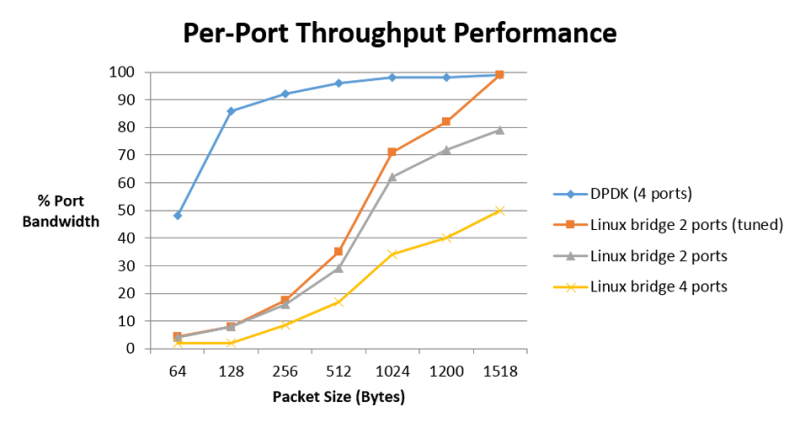
\includegraphics[width=1\textwidth]{img/TB_per-port-throughput-performance-800x428.png}
        \caption{Comparación entre Linux y DPDK. (\ref{bib:img1})}
        \end{center}
    \end{figure}
    
    \pagebreak
    
    \subsection{Funcionamiento Lógico de \textit{DPDK}.}
    \noindent La idea principal de \textit{DPDK} es que una aplicación implementa dichas componentes y librerías que le permiten tomar el control completo de una tarjeta dered  (por simplificar, en este caso es un único RJ45, pero podría ser cualquier interfaz de red o incluso más de una interfaz). Para esta aplicación \textit{DPDK}, el sistema destina un \textit{core} en especifico (\textit{default} 1, pero se puede modificar para asignar más), además de la propia tarjeta de red. Estos recursos de los que la aplicación ha tomado el control, desaparecen del sistema para el usuario, y son dedicados íntegramente para \textit{DPDK}. \\
    
    \noindent Fijándonos directamente en la arquitectura de DPDK, tal y como vemos en \hyperref[bib:link1]{(1)}, la comunicación entre la interfaz de red y la aplicación pasa de estar controlada por el Kernel, a que sea el propio DPDK el encargado de procesar y entender a la interfaz de red. 
    
    \begin{figure}[h]
    	\begin{center}
    		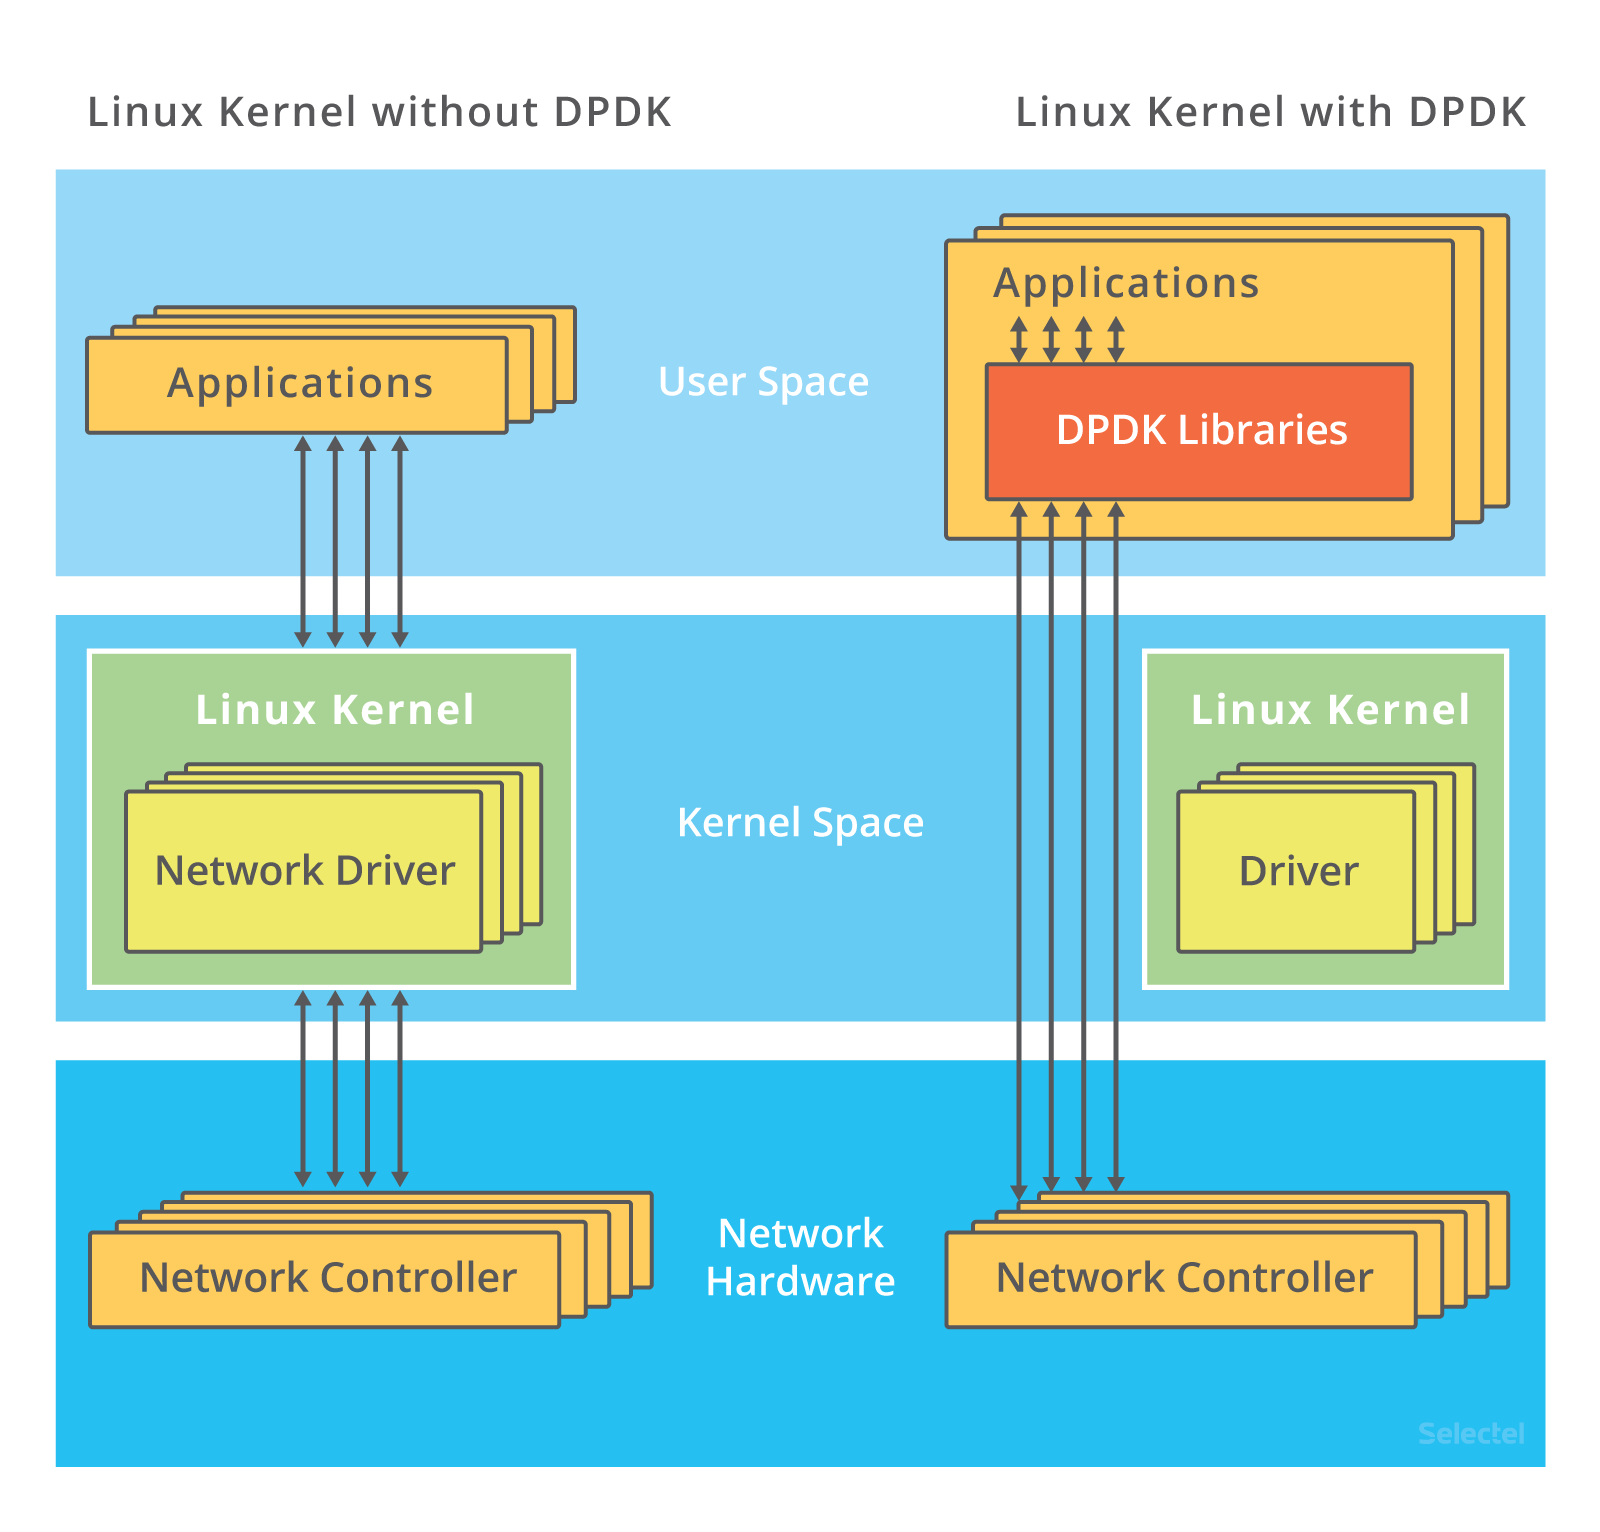
\includegraphics[width=0.5\textwidth]{img/DPDK_Architecture.png}
    		\caption{Comparación entre Linux y DPDK. (\ref{bib:img2})}
    	\end{center}
    \end{figure}

	\noindent Para que esto sea posible, hay otro componente que necesitamos, además de una interfaz de red compatible y una aplicación DPDK. Esto son las huge pages, suponiendo una parte crucial de la aplicación ya que nos permite alojar grandes porciones de datos y nos da la posibilidad de hacer rápidamente a ellos. En el caso de que los paquetes de red sean procesados por el kernel de Linux, utilizamos el acceso a memoría de tipo DMA (\hyperref[bib:img2]{\emph{Direct Memory Access}}) 
	
    
    \pagebreak
    
    \subsection{¿Qué son las \emph{huge pages}?}
    \noindent Para entender correctamente lo que son las \emph{huge pages}, primero tenemos que profundizar en el concepto de \emph{pages}. Cuando un proceso utiliza algo de memoria, la CPU marca la RAM como que está siendo utilizada por dicho proceso. Para aumentar la eficiencia, la CPU asigna la RAM en "porciones" (\emph{chunks}) de 4K bytes (valor \emph{default} en la mayoría de plataformas). Estas porciones se les llama \emph{pages}.\\
    
    \noindent Como el espacio de direccionamiento del proceso es virtual, la CPU y el SO tienen que recordar que páginas pertenecen a que procesos, y además, donde se almacenan. Por consecuencia, cuantas más páginas tengas, más tiempo tardarás en encontrar donde está la memoria alojada. En comparativa, si un proceso utiliza 1GB de memoria, haciendo la cuenta, serían 262144 entradas a comprobar (1GB/4K). Sin embargo, si una \emph{Page Table Entry} utiliza 8 \emph{bytes}, serían 262144 * 8 entradas a comprobar.\\
    
    \noindent La mayoría de CPU actuales soportan páginas de mayor tamaño (por lo que la CPU tiene muchas menos entradas para comprobar), estas pueden recibir el nombre de \emph{Huge pages} (en Linux), \emph{Super pages} (en BSD) o \emph{Larger pages} (en Windows), aunque todas son lo mismo.\\
    
    \subsubsection{Cómo configuramos las \emph{huge pages} para DPDK.}
    \noindent Según la documentación oficial de \hyperref[bib:link4]{\emph{DPDK: Quick Start}}, tenemos que realizar una intervención manual en la instalación de DPDK, en relación a las \emph{huge pages}. Necesitamos "reservar" las \emph{huge pages}, lo haríamos tal que: 
    
    \begin{verbatim}
    	mkdir -p /dev/hugepages
    	mountpoint -q /dev/hugepages || mount -t hugetlbfs nodev /dev/hugepages
    	echo 64 > /sys/devices/system/node/node0/hugepages/hugepages-2048kB/nr_hugepages
    \end{verbatim}

	\pagebreak

	\subsection{Hardware soportado por DPDK.}
	
	\noindent El primer requisito de hardware para poder utilizar DPDK, es estar en disposición de una CPU compatible, aunque es lo común que así sea, es conveniente enumerarlas de cara a futuras aplicaciones. Dichas arquitecturas serían:
	\begin{itemize}
		\item \textbf{x86} (AMD, Intel)
		
		\item \textbf{PPC} (POWER9)
		
		\item \textbf{ARM} (BlueField, DPAA, DPAA2, OCTEON TX, OCTEON TX2)
	\end{itemize}
	
	\noindent En el sentido de las interfaces de red, tenemos mucha más variedad en donde elegir, tanto en lo que a fabricantes se refiere como en drivers de las propias tarjetas. Es importante tener en cuenta esta lista (y revisar adecuadamente la documentación de DPDK (\hyperref[bib:link6]{\textit{Supported Hardware}})) ya que dependiendo de la controladora que utilicemos, el driver puede tener funcionalidades específicas, además de cambiar los parámetros básicos que podemos entender como normales en dicha controladora (velocidad de transferencias, usar RJ-45 o utilizar fibra...). Siendo recomendable visitar la página oficial, aún podríamos listar las tarjetas de red compatibles con DPDK, siendo esa lista la siguiente:

	\begin{multicols}{2}
		\begin{itemize}
			\item AMD
			\item Amazon
			\item Aquantia
			\item Atomic Rules
			\item Broadcom
			\item Chelsio
			\item Cisco
			\item Hisilicon
			\item Huawei
			\item Intel
			\item Marvell
			\item Mellanox
			\item NXP
			\item Netcope
			\item Netronome
			\item Solarflare
			\item Wangxun
			\item \textit{Software NICs}
		\end{itemize}
	\end{multicols}

	\noindent Como podemos comprobar, la lista de fabricantes que tienen NICs compatibles con DPDK es amplia. Por hacer más liviana la comprensión de los conceptos, podríamos destacar los siguientes fabricantes:
	\begin{itemize}
		\item Intel
		\item \textit{Software NICs}
	\end{itemize}

	\pagebreak
	
	\noindent En el caso de Intel, es importante destacarle sobre todo ya que además de tener muchas drivers para una gran variedad de tarjetas de red, fue el precursor de DPDK. Al tener ya un rodaje, la mayoría de sus drivers tienen ya un recorrido por parte de la comunidad, situándolos como una opción muy competitiva respecto al resto de controladores.\\
	
	 \noindent Por otro lado, los \textit{Software NICs} son importantes ya que, aunque no son un fabricante específico, nos permite utilizar un mínimo kernel de Linux para pasar la información de un controlador no soportado por DPDK, pero que tras estos controladores, si que puedan ser utilizados por aplicaciones DPDK. \\
	 
	 \noindent Centrándonos de manera específica en estos dos fabricantes, podemos hacer una enumeración de drivers y de tarjetas soportadas.
	 
	 \begin{itemize}
	 	\item Intel \hyperref[bib:link7]{(\textit{Supported NICs Intel})}
	 	\begin{multicols}{2}
	 		\begin{itemize}
	 			\item e1000 [VM Emulated Devices]
	 			
	 			\item e1000e 
	 			
	 			\item igb [1GbE]
	 			
	 			\item igc [2.5GbE]
	 			
	 			\item ixgbe [10G]
	 			
	 			\item i40e [10/25/40G]
	 			
	 			\item ice [10/25/50/100G]
	 			
	 			\item fm10k [40/100GbE]
	 			
	 			\item ipn3ke [FPGA Controller]
	 			
	 			\item ifc
	 		\end{itemize}
	 	\end{multicols}
	 	
	 	\item Software NICs \hyperref[bib:link8]{(\textit{Supported Software NICs})}
	 	\begin{multicols}{2}
	 		\begin{itemize}
	 			\item AF\_PACKET [AF\_PACKET socket]
	 			
	 			\item AF\_XDP [AF\_XDP socket]
	 			
	 			\item tap/tun [kernel L2/L3]
	 			
	 			\item pcap [file or kernel driver]
	 			
	 			\item ring [memory]
	 			
	 			\item memif [memory]
	 		\end{itemize}
	 	\end{multicols}
	 \end{itemize}
    
    %%% OKO.
    \pagebreak
    \section{OKO}
    
    %%% Glosario
    \pagebreak
    \section{Glosario de términos.}
    \begin{itemize}
    	\item DPDK. \textit{Data Plane Development Kit.}
    	\item NICs. \textit{Network Interface Card.}
    \end{itemize}
    
    
    %%% Bibliography
    \pagebreak
    \section{Bibliografía}
    \subsection{Links and references}
    %%\hyperref[bib:link1]{\emph{Reference of bibliography}}
    \begin{enumerate}
        %1
        \item 
        \label{bib:link1} \href{https://blog.selectel.com/introduction-dpdk-architecture-principles/}{Introduction to DPDK: Architecture and Principles}
        
        %2
        \item 
        \label{bib:link2}\href{https://en.wikipedia.org/wiki/Data_Plane_Development_Kit}{Wikipedia: Data Plane Development Kit}
        
        %3
        \item 
        \label{bib:link3}\href{https://wiki.debian.org/Hugepages}{Hugepages}
        
        %4
        \item
        \label{bib:link4}\href{https://core.dpdk.org/doc/quick-start/}{DPDK: Quick Start}
        
        %5
        \item
        \label{bib:link5} \href{https://techopedia.com/definition/2767/direct-memory-access-dma}{Direct Memory Access (DMA)}
        
        %6
        \item
        \label{bib:link6} \href{https://core.dpdk.org/supported/}{Lista de arquitecturas e interfaces de red soportadas por DPDK.}
        
        %7
        \item
        \label{bib:link7} \href{https://core.dpdk.org/supported/nics/intel/}{NICs de Intel soportados por DPDK}
        
        %8
        \item
        \label{bib:link8} \href{https://core.dpdk.org/supported/nics/sw/}{Software NICs soportados por DPDK}
    \end{enumerate}

	\subsection{Images}
	\begin{enumerate}
		%1
		\item 
		\label{bib:img1}\href{https://www.accton.com/Technology-Brief/intel-dpdk-performance-on-the-sau5081i-server/}{Imagen comparativa de BW en diferentes tests case.}
		
		%2
		\item
		\label{bib:img2} \href{https://blog.selectel.com/introduction-dpdk-architecture-principles/}{DPDK: How it works. General Features}
		
		
	\end{enumerate}
	
\end{document}